% 2007 浙江卷文 第21题 图 (single_conic_lines)
% ellipse x^2/4 + y^2 = 1; chord AB (schematic) y=0.5335x+0.5519; segments OA, OB
\usetikzlibrary{arrows.meta,calc}
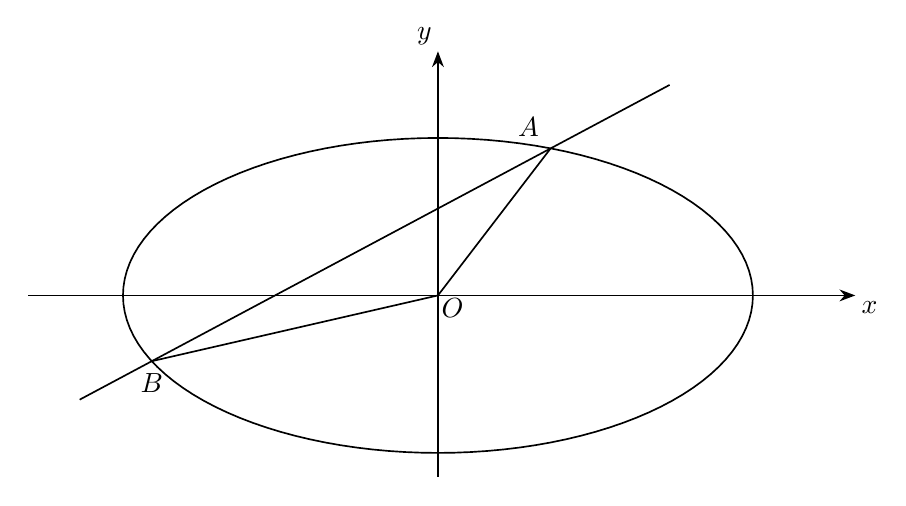
\begin{tikzpicture}[x=2cm,y=2cm,line width=.6pt,font=\normalsize,>=Stealth]
  % axes
  \draw[->] (-2.6,0) -- (2.65,0) node[below right=2pt,inner sep=0pt] {$x$};
  \draw[->] (0,-1.15) -- (0,1.55) node[above left=2pt,inner sep=0pt] {$y$};
  % ellipse x^2/4 + y^2 = 1
  \draw plot[domain=0:360,samples=121,variable=\t] ({2*cos(\t)},{1*sin(\t)});
  % chord AB extended beyond A and B
  \coordinate (C1) at (-2.275,-0.6618);
  \coordinate (C2) at (1.471,1.3367);
  \draw (C1) -- (C2);
  % intersections A (Q1), B (Q3)
  \coordinate (A) at (0.7157,0.9338);
  \coordinate (B) at (-1.8173,-0.4176);
  % triangle sides
  \draw (0,0) -- (A);
  \draw (0,0) -- (B);
  % labels
  \node[above left=4pt,inner sep=0pt] at (A) {$A$};
  \node[below=4pt,inner sep=0pt] at (B) {$B$};
  \node[below right=1pt,inner sep=0pt] at (0,0) {$O$};
\end{tikzpicture}
